% !Mode:: "TeX:UTF-8"
\chapter{系统测试}


\section{部署本地测试}

部署到本地的实验主要验证平台部署到本地的功能的正确性,同时分别把模型部署到CPU和Cuda的计算平台上,分别验证不同的推理时间。

\subsection{测试环境}

模型部署的本地电脑采用的是64位的Ubuntu系统,使用intel i5 10210U CPU,Nvidia MX250 GPU。


\subsection{测试流程}

首先,从torchvison库中获得预训练的resnet18模型。

其次,使用该平台的接口,将模型部署到本地设备上,分别使用CPU和GPU进行计算。

最后,分别使用CPU和GPU执行推理100次,记录执行的时间。

\subsection{测试结果}

\begin{figure}[h!]
    \centering
    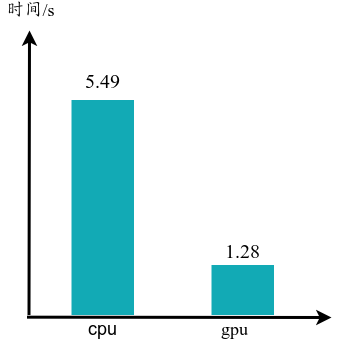
\includegraphics[width=180bp]{figure/expr_local.png}
    \caption{本地测试结果}
    \label{expr_local}
\end{figure}

如上图\ref{expr_local}所示,可以看到,部署到本地的模型在CPU和GPU上分别执行100次推理时,GPU只需要1.28秒而CPU需要5.49秒。


\section{部署安卓测试}

部署到安卓的实验来验证本地主机与按住设备的通信是否正常,同时验证该平台部署到安卓设备的功能的正确性。该实验分别把模型部署到安卓端的CPU,OpenCL,Vulkan计算平台上,验证每种计算平台执行推理的时间。

\subsection{测试环境}

本实验的本地端采用64位Ubuntu系统,使用intel i5 10210U CPU,Nvidia MX250 GPU。安卓端是使用android11系统,使用MTK Helio G90T CPU,ARM Mali G76 MC4 GPU。


\subsection{测试流程}

首先,使用torchvision库获得预训练的resnet18模型。

其次,使用平台的接口把模型部署到安卓设备上,同时在安卓端使用前文构建的App,输入指定的ip,port,key来打开Rpc通信。同时可以使用命令python -m tvm.exec.query\_rpc\_tracker --host=host --port=port来检验安卓设备是否连接到了本地电脑。

最后,分别使用CPU,OpenCL,Vulkan执行推理,记录执行时间。


\subsection{测试结果}

\begin{figure}[h!]
    \centering
    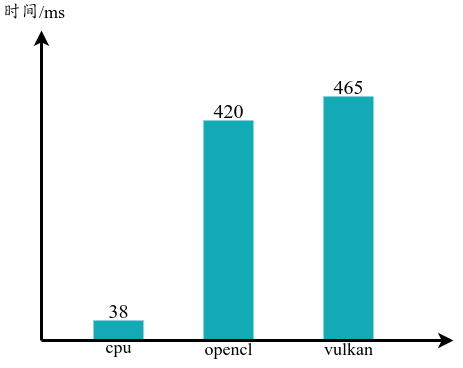
\includegraphics[width=180bp]{figure/expr_android.png}
    \caption{安卓测试结果}
    \label{expr_android}
\end{figure}

如上图\ref{expr_android}所示,虽然在安卓设备上使用了GPU,但是反而比CPU慢,因为TVM没有针对该GPU的优化,所以导致了执行速度下降明显。


\section{部署树莓派测试}

部署到树莓派的测试主要验证平台是否能够正常的部署到树莓派设备上,因为树莓派设备上只有CPU处理器,所以该部分的测试只测试功能的正确性。

\subsection{测试环境}

模型编译采用的本地环境为64位Ubuntu系统,使用intel i5 10210U CPU,Nvidia MX250 GPU。模型执行的树莓派采用的是ARM架构的CPU。


\subsection{测试流程}

首先,通过Pytorch的预训练仓库,获得Resnet18的预训练模型。

\begin{figure}[h!]
    \centering
    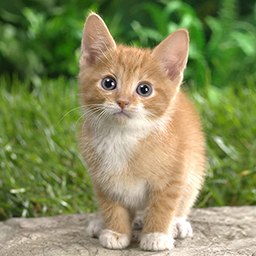
\includegraphics[width=180bp]{figure/cat.png}
    \caption{测试图片}
    \label{cat}
\end{figure}

其次,下载Imagenet1000分类的标签文件。并选取一张测试图片\ref{cat}。

最后,使用该平台的接口部署模型到树莓派设备进行推理,并预测测试图片的类别。


\subsection{测试结果}

\begin{figure}
    \centering
    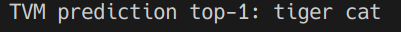
\includegraphics[width=180bp]{figure/expr_rasp.png}
    \caption{树莓派测试结果}
    \label{expr_rasp}
\end{figure}

如上图\ref{expr_rasp}所示,通过接口部署的模型得到了正确的预测结果。


\section{部署VTA测试}

与部署到树莓派相同,本测试主要验证能否通过本平台提供的接口将模型在VTA模拟器上执行。

\subsection{测试环境}

模型编译参用的本地环境为64位Ubuntu系统,使用intel i5 10210U CPU,Nvidia MX250 GPU。VTA模拟器采用的参数配置如下:
\begin{itemize}
    \item {TARGET:sim。}
    \item {LOG\_INP\_WIDTH:3。}
    \item {LOG\_WGT\_WIDTH:3。}
    \item {LOG\_ACC\_WIDTH:5。}
    \item {LOG\_BATCH:0。}
    \item {LOG\_BLOCK:4。}
    \item {LOG\_UOP\_BUFF\_SIZE:5。}
    \item {LOG\_INP\_BUFF\_SIZE:15。}
    \item {LOG\_WGT\_BUFF\_SIZE:18。}
    \item {LOG\_ACC\_BUFF\_SIZE:17。}
\end{itemize}


\subsection{测试流程}

首先,通过Pytorch的预训练仓库,获得Resnet18的预训练模型。

其次,下载Imagenet1000分类的标签文件。并选取一张测试图片\ref{cat}。

最后,使用该平台的接口部署模型到VTA模拟器进行推理,并预测测试图片的类别。


\subsection{测试结果}

\begin{figure}
    \centering
    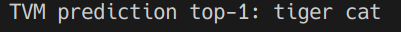
\includegraphics[width=180bp]{figure/expr_rasp.png}
    \caption{树莓派测试结果}
    \label{expr_vta}
\end{figure}

如上图\ref{expr_vta}所示,通过接口部署的模型得到了正确的预测结果。